\documentclass[1p]{elsarticle_modified}
%\bibliographystyle{elsarticle-num}

%\usepackage[colorlinks]{hyperref}
%\usepackage{abbrmath_seonhwa} %\Abb, \Ascr, \Acal ,\Abf, \Afrak
\usepackage{amsfonts}
\usepackage{amssymb}
\usepackage{amsmath}
\usepackage{amsthm}
\usepackage{scalefnt}
\usepackage{amsbsy}
\usepackage{kotex}
\usepackage{caption}
\usepackage{subfig}
\usepackage{color}
\usepackage{graphicx}
\usepackage{xcolor} %% white, black, red, green, blue, cyan, magenta, yellow
\usepackage{float}
\usepackage{setspace}
\usepackage{hyperref}

\usepackage{tikz}
\usetikzlibrary{arrows}

\usepackage{multirow}
\usepackage{array} % fixed length table
\usepackage{hhline}

%%%%%%%%%%%%%%%%%%%%%
\makeatletter
\renewcommand*\env@matrix[1][\arraystretch]{%
	\edef\arraystretch{#1}%
	\hskip -\arraycolsep
	\let\@ifnextchar\new@ifnextchar
	\array{*\c@MaxMatrixCols c}}
\makeatother %https://tex.stackexchange.com/questions/14071/how-can-i-increase-the-line-spacing-in-a-matrix
%%%%%%%%%%%%%%%

\usepackage[normalem]{ulem}

\newcommand{\msout}[1]{\ifmmode\text{\sout{\ensuremath{#1}}}\else\sout{#1}\fi}
%SOURCE: \msout is \stkout macro in https://tex.stackexchange.com/questions/20609/strikeout-in-math-mode

\newcommand{\cancel}[1]{
	\ifmmode
	{\color{red}\msout{#1}}
	\else
	{\color{red}\sout{#1}}
	\fi
}

\newcommand{\add}[1]{
	{\color{blue}\uwave{#1}}
}

\newcommand{\replace}[2]{
	\ifmmode
	{\color{red}\msout{#1}}{\color{blue}\uwave{#2}}
	\else
	{\color{red}\sout{#1}}{\color{blue}\uwave{#2}}
	\fi
}

\newcommand{\Sol}{\mathcal{S}} %segment
\newcommand{\D}{D} %diagram
\newcommand{\A}{\mathcal{A}} %arc


%%%%%%%%%%%%%%%%%%%%%%%%%%%%%5 test

\def\sl{\operatorname{\textup{SL}}(2,\Cbb)}
\def\psl{\operatorname{\textup{PSL}}(2,\Cbb)}
\def\quan{\mkern 1mu \triangleright \mkern 1mu}

\theoremstyle{definition}
\newtheorem{thm}{Theorem}[section]
\newtheorem{prop}[thm]{Proposition}
\newtheorem{lem}[thm]{Lemma}
\newtheorem{ques}[thm]{Question}
\newtheorem{cor}[thm]{Corollary}
\newtheorem{defn}[thm]{Definition}
\newtheorem{exam}[thm]{Example}
\newtheorem{rmk}[thm]{Remark}
\newtheorem{alg}[thm]{Algorithm}

\newcommand{\I}{\sqrt{-1}}
\begin{document}

%\begin{frontmatter}
%
%\title{Boundary parabolic representations of knots up to 8 crossings}
%
%%% Group authors per affiliation:
%\author{Yunhi Cho} 
%\address{Department of Mathematics, University of Seoul, Seoul, Korea}
%\ead{yhcho@uos.ac.kr}
%
%
%\author{Seonhwa Kim} %\fnref{s_kim}}
%\address{Center for Geometry and Physics, Institute for Basic Science, Pohang, 37673, Korea}
%\ead{ryeona17@ibs.re.kr}
%
%\author{Hyuk Kim}
%\address{Department of Mathematical Sciences, Seoul National University, Seoul 08826, Korea}
%\ead{hyukkim@snu.ac.kr}
%
%\author{Seokbeom Yoon}
%\address{Department of Mathematical Sciences, Seoul National University, Seoul, 08826,  Korea}
%\ead{sbyoon15@snu.ac.kr}
%
%\begin{abstract}
%We find all boundary parabolic representation of knots up to 8 crossings.
%
%\end{abstract}
%\begin{keyword}
%    \MSC[2010] 57M25 
%\end{keyword}
%
%\end{frontmatter}

%\linenumbers
%\tableofcontents
%
\newcommand\colored[1]{\textcolor{white}{\rule[-0.35ex]{0.8em}{1.4ex}}\kern-0.8em\color{red} #1}%
%\newcommand\colored[1]{\textcolor{white}{ #1}\kern-2.17ex	\textcolor{white}{ #1}\kern-1.81ex	\textcolor{white}{ #1}\kern-2.15ex\color{red}#1	}

{\Large $\underline{8_{15}~(K8a_{2})}$}

\setlength{\tabcolsep}{10pt}
\renewcommand{\arraystretch}{1.6}
\vspace{1cm}\begin{tabular}{m{100pt}>{\centering\arraybackslash}m{274pt}}
\multirow{5}{120pt}{
	\centering
	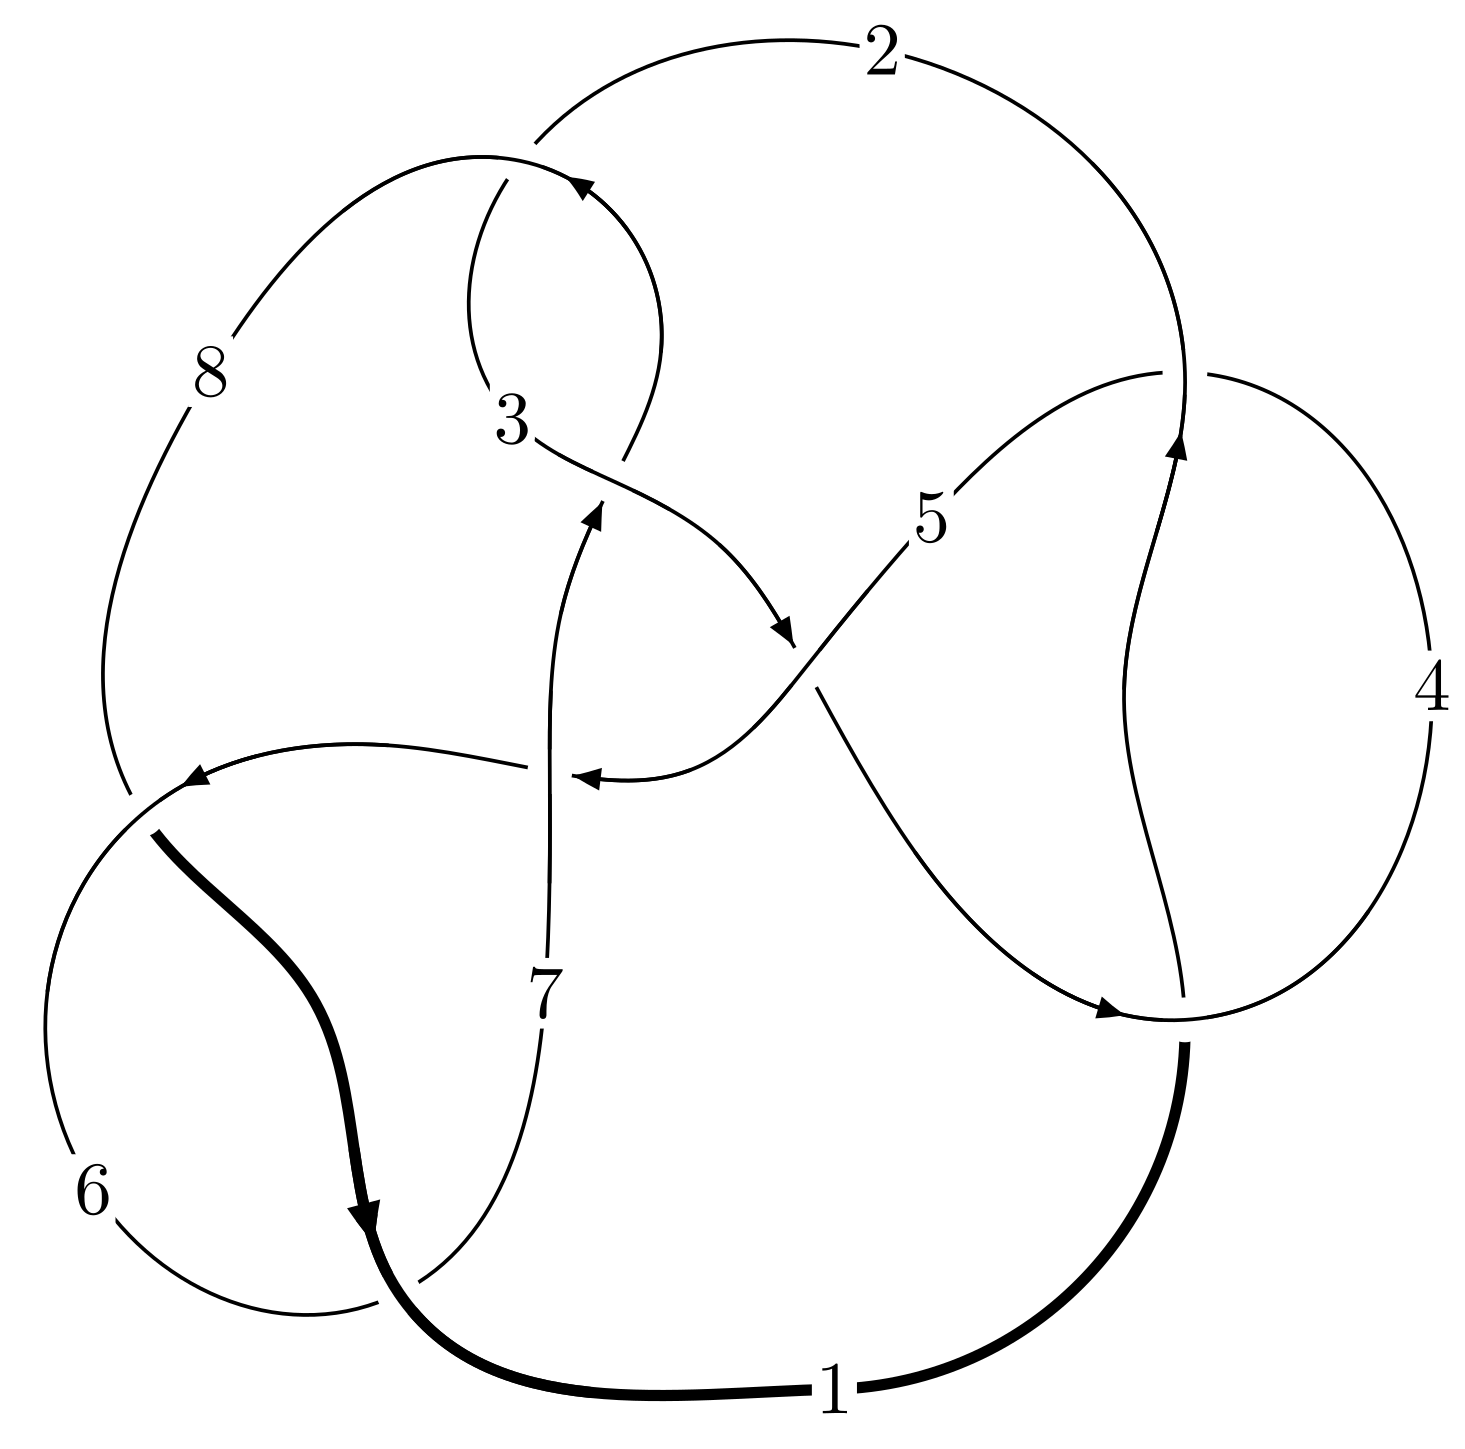
\includegraphics[width=112pt]{../../../GIT/diagram.site/Diagrams/png/29_8_15.png}\\
\ \ \ A knot diagram\footnotemark}&
\allowdisplaybreaks
\textbf{Linearized knot diagam} \\
\cline{2-2}
 &
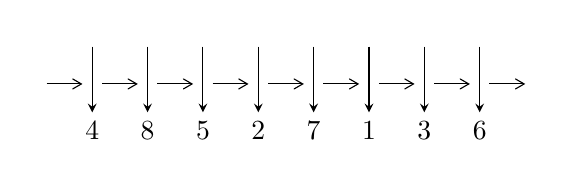
\begin{tikzpicture}[x=20pt, y=17pt]
	% nodes
	\node (C0) at (0, 0) {};
	\node (C1) at (1, 0) {};
	\node (C1U) at (1, +1) {};
	\node (C1D) at (1, -1) {4};

	\node (C2) at (2, 0) {};
	\node (C2U) at (2, +1) {};
	\node (C2D) at (2, -1) {8};

	\node (C3) at (3, 0) {};
	\node (C3U) at (3, +1) {};
	\node (C3D) at (3, -1) {5};

	\node (C4) at (4, 0) {};
	\node (C4U) at (4, +1) {};
	\node (C4D) at (4, -1) {2};

	\node (C5) at (5, 0) {};
	\node (C5U) at (5, +1) {};
	\node (C5D) at (5, -1) {7};

	\node (C6) at (6, 0) {};
	\node (C6U) at (6, +1) {};
	\node (C6D) at (6, -1) {1};

	\node (C7) at (7, 0) {};
	\node (C7U) at (7, +1) {};
	\node (C7D) at (7, -1) {3};

	\node (C8) at (8, 0) {};
	\node (C8U) at (8, +1) {};
	\node (C8D) at (8, -1) {6};
	\node (C9) at (9, 0) {};

	% arrows
	\draw[->,>={angle 60}]
	(C0) edge (C1) (C1) edge (C2) (C2) edge (C3) (C3) edge (C4) (C4) edge (C5) (C5) edge (C6) (C6) edge (C7) (C7) edge (C8) (C8) edge (C9) ;	\draw[->,>=stealth]
	(C1U) edge (C1D) (C2U) edge (C2D) (C3U) edge (C3D) (C4U) edge (C4D) (C5U) edge (C5D) (C6U) edge (C6D) (C7U) edge (C7D) (C8U) edge (C8D) ;
	\end{tikzpicture} \\
\hhline{~~} \\& 
\textbf{Solving Sequence} \\ \cline{2-2} 
 &
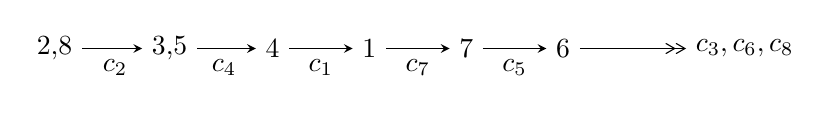
\begin{tikzpicture}[x=35pt, y=7pt]
	% node
	\node (A0) at (-1/8, 0) {2,8};
	\node (A1) at (17/16, 0) {3,5};
	\node (A2) at (17/8, 0) {4};
	\node (A3) at (25/8, 0) {1};
	\node (A4) at (33/8, 0) {7};
	\node (A5) at (41/8, 0) {6};
	\node (C1) at (1/2, -1) {$c_{2}$};
	\node (C2) at (13/8, -1) {$c_{4}$};
	\node (C3) at (21/8, -1) {$c_{1}$};
	\node (C4) at (29/8, -1) {$c_{7}$};
	\node (C5) at (37/8, -1) {$c_{5}$};
	\node (A6) at (7, 0) {$c_{3},c_{6},c_{8}$};

	% edge
	\draw[->,>=stealth]	
	(A0) edge (A1) (A1) edge (A2) (A2) edge (A3) (A3) edge (A4) (A4) edge (A5) ;
	\draw[->>,>={angle 60}]	
	(A5) edge (A6);
\end{tikzpicture} \\ 

\end{tabular} \\

\footnotetext{
The image of knot diagram is generated by the software ``\textbf{Draw programme}" developed by Andrew Bartholomew(\url{http://www.layer8.co.uk/maths/draw/index.htm\#Running-draw}), where we modified some parts for our purpose(\url{https://github.com/CATsTAILs/LinksPainter}).
}\phantom \\ \newline 
\centering \textbf{Ideals for irreducible components\footnotemark of $X_{\text{par}}$} 
 
\begin{align*}
I^u_{1}&=\langle 
u^6-2 u^5+3 u^4-2 u^3+b+u-1,\;- u^6+3 u^5-4 u^4+3 u^3- u^2+2 a- u,\\
\phantom{I^u_{1}}&\phantom{= \langle  }u^7-3 u^6+6 u^5-7 u^4+5 u^3- u^2-2 u+2\rangle \\
I^u_{2}&=\langle 
u^4 a+u^2 a+u^3- a u+b+a+u-1,\;- u^3 a-2 u^2 a+u^3+a^2-2 a u+u^2-2 a+u+1,\\
\phantom{I^u_{2}}&\phantom{= \langle  }u^5+u^4+2 u^3+u^2+u+1\rangle \\
\\
I^v_{1}&=\langle 
a,\;b-1,\;v+1\rangle \\
\end{align*}
\raggedright * 3 irreducible components of $\dim_{\mathbb{C}}=0$, with total 18 representations.\\
\footnotetext{All coefficients of polynomials are rational numbers. But the coefficients are sometimes approximated in decimal forms when there is not enough margin.}
\newpage
\renewcommand{\arraystretch}{1}
\centering \section*{I. $I^u_{1}= \langle u^6-2 u^5+3 u^4-2 u^3+b+u-1,\;- u^6+3 u^5-4 u^4+3 u^3- u^2+2 a- u,\;u^7-3 u^6+6 u^5-7 u^4+5 u^3- u^2-2 u+2 \rangle$}
\flushleft \textbf{(i) Arc colorings}\\
\begin{tabular}{m{7pt} m{180pt} m{7pt} m{180pt} }
\flushright $a_{2}=$&$\begin{pmatrix}1\\0\end{pmatrix}$ \\
\flushright $a_{8}=$&$\begin{pmatrix}0\\u\end{pmatrix}$ \\
\flushright $a_{3}=$&$\begin{pmatrix}1\\u^2\end{pmatrix}$ \\
\flushright $a_{5}=$&$\begin{pmatrix}\frac{1}{2} u^6-\frac{3}{2} u^5+\cdots+\frac{1}{2} u^2+\frac{1}{2} u\\- u^6+2 u^5-3 u^4+2 u^3- u+1\end{pmatrix}$ \\
\flushright $a_{4}=$&$\begin{pmatrix}-\frac{1}{2} u^6+\frac{1}{2} u^5+\cdots-\frac{1}{2} u+1\\- u^6+2 u^5-3 u^4+2 u^3- u+1\end{pmatrix}$ \\
\flushright $a_{1}=$&$\begin{pmatrix}\frac{1}{2} u^6-\frac{3}{2} u^5+\cdots+\frac{1}{2} u-1\\u^4- u^3+u^2-1\end{pmatrix}$ \\
\flushright $a_{7}=$&$\begin{pmatrix}u\\u^3+u\end{pmatrix}$ \\
\flushright $a_{6}=$&$\begin{pmatrix}\frac{1}{2} u^6-\frac{1}{2} u^5+\cdots+\frac{1}{2} u^2-\frac{1}{2} u\\u^6-2 u^5+3 u^4-3 u^3+u^2-1\end{pmatrix}$\\&\end{tabular}
\flushleft \textbf{(ii) Obstruction class $= -1$}\\~\\
\flushleft \textbf{(iii) Cusp Shapes $= 2 u^6-8 u^5+10 u^4-10 u^3+4 u-12$}\\~\\
\newpage\renewcommand{\arraystretch}{1}
\flushleft \textbf{(iv) u-Polynomials at the component}\newline \\
\begin{tabular}{m{50pt}|m{274pt}}
Crossings & \hspace{64pt}u-Polynomials at each crossing \\
\hline $$\begin{aligned}c_{1},c_{4},c_{6}\\c_{8}\end{aligned}$$&$\begin{aligned}
&u^7- u^6- u^5+2 u^4+u^3-2 u^2+u+1
\end{aligned}$\\
\hline $$\begin{aligned}c_{2},c_{7}\end{aligned}$$&$\begin{aligned}
&u^7-3 u^6+6 u^5-7 u^4+5 u^3- u^2-2 u+2
\end{aligned}$\\
\hline $$\begin{aligned}c_{3},c_{5}\end{aligned}$$&$\begin{aligned}
&u^7+3 u^6+7 u^5+8 u^4+9 u^3+6 u^2+5 u+1
\end{aligned}$\\
\hline
\end{tabular}\\~\\
\newpage\renewcommand{\arraystretch}{1}
\flushleft \textbf{(v) Riley Polynomials at the component}\newline \\
\begin{tabular}{m{50pt}|m{274pt}}
Crossings & \hspace{64pt}Riley Polynomials at each crossing \\
\hline $$\begin{aligned}c_{1},c_{4},c_{6}\\c_{8}\end{aligned}$$&$\begin{aligned}
&y^7-3 y^6+7 y^5-8 y^4+9 y^3-6 y^2+5 y-1
\end{aligned}$\\
\hline $$\begin{aligned}c_{2},c_{7}\end{aligned}$$&$\begin{aligned}
&y^7+3 y^6+4 y^5+y^4- y^3+7 y^2+8 y-4
\end{aligned}$\\
\hline $$\begin{aligned}c_{3},c_{5}\end{aligned}$$&$\begin{aligned}
&y^7+5 y^6+19 y^5+36 y^4+49 y^3+38 y^2+13 y-1
\end{aligned}$\\
\hline
\end{tabular}\\~\\
\newpage\flushleft \textbf{(vi) Complex Volumes and Cusp Shapes}
$$\begin{array}{c|c|c}  
\text{Solutions to }I^u_{1}& \I (\text{vol} + \sqrt{-1}CS) & \text{Cusp shape}\\
 \hline 
\begin{aligned}
u &= \phantom{-}0.984140 + 0.426152 I \\
a &= \phantom{-}0.472917 + 0.120643 I \\
b &= \phantom{-}0.985336 - 0.506466 I\end{aligned}
 & -2.09542 + 3.93070 I & -10.25941 - 4.87230 I \\ \hline\begin{aligned}
u &= \phantom{-}0.984140 - 0.426152 I \\
a &= \phantom{-}0.472917 - 0.120643 I \\
b &= \phantom{-}0.985336 + 0.506466 I\end{aligned}
 & -2.09542 - 3.93070 I & -10.25941 + 4.87230 I \\ \hline\begin{aligned}
u &= \phantom{-}0.167785 + 1.218780 I \\
a &= \phantom{-}0.529166 - 1.016880 I \\
b &= -0.597306 + 0.773845 I\end{aligned}
 & \phantom{-}3.85236 + 0.95540 I & -3.31071 - 2.37083 I \\ \hline\begin{aligned}
u &= \phantom{-}0.167785 - 1.218780 I \\
a &= \phantom{-}0.529166 + 1.016880 I \\
b &= -0.597306 - 0.773845 I\end{aligned}
 & \phantom{-}3.85236 - 0.95540 I & -3.31071 + 2.37083 I \\ \hline\begin{aligned}
u &= \phantom{-}0.654547 + 1.202470 I \\
a &= -0.33478 + 1.51279 I \\
b &= -1.139460 - 0.630170 I\end{aligned}
 & \phantom{-}0.36369 - 9.93065 I & -8.46028 + 7.33664 I \\ \hline\begin{aligned}
u &= \phantom{-}0.654547 - 1.202470 I \\
a &= -0.33478 - 1.51279 I \\
b &= -1.139460 + 0.630170 I\end{aligned}
 & \phantom{-}0.36369 + 9.93065 I & -8.46028 - 7.33664 I \\ \hline\begin{aligned}
u &= -0.612945\phantom{ +0.000000I} \\
a &= \phantom{-}0.665400\phantom{ +0.000000I} \\
b &= \phantom{-}0.502855\phantom{ +0.000000I}\end{aligned}
 & -0.951399\phantom{ +0.000000I} & -9.93920\phantom{ +0.000000I}\\
 \hline 
 \end{array}$$\newpage\newpage\renewcommand{\arraystretch}{1}
\centering \section*{II. $I^u_{2}= \langle u^4 a+u^2 a+u^3- a u+b+a+u-1,\;- u^3 a+u^3+\cdots-2 a+1,\;u^5+u^4+2 u^3+u^2+u+1 \rangle$}
\flushleft \textbf{(i) Arc colorings}\\
\begin{tabular}{m{7pt} m{180pt} m{7pt} m{180pt} }
\flushright $a_{2}=$&$\begin{pmatrix}1\\0\end{pmatrix}$ \\
\flushright $a_{8}=$&$\begin{pmatrix}0\\u\end{pmatrix}$ \\
\flushright $a_{3}=$&$\begin{pmatrix}1\\u^2\end{pmatrix}$ \\
\flushright $a_{5}=$&$\begin{pmatrix}a\\- u^4 a- u^2 a- u^3+a u- a- u+1\end{pmatrix}$ \\
\flushright $a_{4}=$&$\begin{pmatrix}- u^4 a- u^2 a- u^3+a u- u+1\\- u^4 a- u^2 a- u^3+a u- a- u+1\end{pmatrix}$ \\
\flushright $a_{1}=$&$\begin{pmatrix}u^4 a+2 u^2 a+u^3- a u+2 a+u-1\\u^4 a+2 u^2 a+u^3- a u+a+u-1\end{pmatrix}$ \\
\flushright $a_{7}=$&$\begin{pmatrix}u\\u^3+u\end{pmatrix}$ \\
\flushright $a_{6}=$&$\begin{pmatrix}u^4 a- u^4+2 u^2 a- u^3-2 u^2+2 a- u-1\\u^4 a+u^3 a- u^4+2 u^2 a-2 u^3+a u-2 u^2+a- u\end{pmatrix}$\\&\end{tabular}
\flushleft \textbf{(ii) Obstruction class $= -1$}\\~\\
\flushleft \textbf{(iii) Cusp Shapes $= 4 u^3+4 u^2+4 u-6$}\\~\\
\newpage\renewcommand{\arraystretch}{1}
\flushleft \textbf{(iv) u-Polynomials at the component}\newline \\
\begin{tabular}{m{50pt}|m{274pt}}
Crossings & \hspace{64pt}u-Polynomials at each crossing \\
\hline $$\begin{aligned}c_{1},c_{4},c_{6}\\c_{8}\end{aligned}$$&$\begin{aligned}
&u^{10}- u^9-2 u^8+4 u^7-4 u^5+3 u^4+u^3-2 u^2+1
\end{aligned}$\\
\hline $$\begin{aligned}c_{2},c_{7}\end{aligned}$$&$\begin{aligned}
&(u^5+u^4+2 u^3+u^2+u+1)^2
\end{aligned}$\\
\hline $$\begin{aligned}c_{3},c_{5}\end{aligned}$$&$\begin{aligned}
&u^{10}+5 u^9+\cdots+4 u+1
\end{aligned}$\\
\hline
\end{tabular}\\~\\
\newpage\renewcommand{\arraystretch}{1}
\flushleft \textbf{(v) Riley Polynomials at the component}\newline \\
\begin{tabular}{m{50pt}|m{274pt}}
Crossings & \hspace{64pt}Riley Polynomials at each crossing \\
\hline $$\begin{aligned}c_{1},c_{4},c_{6}\\c_{8}\end{aligned}$$&$\begin{aligned}
&y^{10}-5 y^9+\cdots-4 y+1
\end{aligned}$\\
\hline $$\begin{aligned}c_{2},c_{7}\end{aligned}$$&$\begin{aligned}
&(y^5+3 y^4+4 y^3+y^2- y-1)^2
\end{aligned}$\\
\hline $$\begin{aligned}c_{3},c_{5}\end{aligned}$$&$\begin{aligned}
&y^{10}- y^9-6 y^7+22 y^6+6 y^5+45 y^4+15 y^3+22 y^2+4 y+1
\end{aligned}$\\
\hline
\end{tabular}\\~\\
\newpage\flushleft \textbf{(vi) Complex Volumes and Cusp Shapes}
$$\begin{array}{c|c|c}  
\text{Solutions to }I^u_{2}& \I (\text{vol} + \sqrt{-1}CS) & \text{Cusp shape}\\
 \hline 
\begin{aligned}
u &= \phantom{-}0.339110 + 0.822375 I \\
a &= \phantom{-}0.445032 + 0.031192 I \\
b &= \phantom{-}1.236040 - 0.156723 I\end{aligned}
 & -2.96077 - 1.53058 I & -9.48489 + 4.43065 I \\ \hline\begin{aligned}
u &= \phantom{-}0.339110 + 0.822375 I \\
a &= \phantom{-}0.46155 + 2.45660 I \\
b &= -0.926127 - 0.393188 I\end{aligned}
 & -2.96077 - 1.53058 I & -9.48489 + 4.43065 I \\ \hline\begin{aligned}
u &= \phantom{-}0.339110 - 0.822375 I \\
a &= \phantom{-}0.445032 - 0.031192 I \\
b &= \phantom{-}1.236040 + 0.156723 I\end{aligned}
 & -2.96077 + 1.53058 I & -9.48489 - 4.43065 I \\ \hline\begin{aligned}
u &= \phantom{-}0.339110 - 0.822375 I \\
a &= \phantom{-}0.46155 - 2.45660 I \\
b &= -0.926127 + 0.393188 I\end{aligned}
 & -2.96077 + 1.53058 I & -9.48489 - 4.43065 I \\ \hline\begin{aligned}
u &= -0.766826\phantom{ +0.000000I} \\
a &= \phantom{-}0.595741 + 0.124010 I \\
b &= \phantom{-}0.608868 - 0.334904 I\end{aligned}
 & -0.888787\phantom{ +0.000000I} & -8.51890\phantom{ +0.000000I} \\ \hline\begin{aligned}
u &= -0.766826\phantom{ +0.000000I} \\
a &= \phantom{-}0.595741 - 0.124010 I \\
b &= \phantom{-}0.608868 + 0.334904 I\end{aligned}
 & -0.888787\phantom{ +0.000000I} & -8.51890\phantom{ +0.000000I} \\ \hline\begin{aligned}
u &= -0.455697 + 1.200150 I \\
a &= \phantom{-}0.542114 + 0.781069 I \\
b &= -0.400287 - 0.864056 I\end{aligned}
 & \phantom{-}2.58269 + 4.40083 I & -5.25569 - 3.49859 I \\ \hline\begin{aligned}
u &= -0.455697 + 1.200150 I \\
a &= -0.04444 - 1.54938 I \\
b &= -1.018500 + 0.644891 I\end{aligned}
 & \phantom{-}2.58269 + 4.40083 I & -5.25569 - 3.49859 I \\ \hline\begin{aligned}
u &= -0.455697 - 1.200150 I \\
a &= \phantom{-}0.542114 - 0.781069 I \\
b &= -0.400287 + 0.864056 I\end{aligned}
 & \phantom{-}2.58269 - 4.40083 I & -5.25569 + 3.49859 I \\ \hline\begin{aligned}
u &= -0.455697 - 1.200150 I \\
a &= -0.04444 + 1.54938 I \\
b &= -1.018500 - 0.644891 I\end{aligned}
 & \phantom{-}2.58269 - 4.40083 I & -5.25569 + 3.49859 I\\
 \hline 
 \end{array}$$\newpage\newpage\renewcommand{\arraystretch}{1}
\centering \section*{III. $I^v_{1}= \langle a,\;b-1,\;v+1 \rangle$}
\flushleft \textbf{(i) Arc colorings}\\
\begin{tabular}{m{7pt} m{180pt} m{7pt} m{180pt} }
\flushright $a_{2}=$&$\begin{pmatrix}1\\0\end{pmatrix}$ \\
\flushright $a_{8}=$&$\begin{pmatrix}-1\\0\end{pmatrix}$ \\
\flushright $a_{3}=$&$\begin{pmatrix}1\\0\end{pmatrix}$ \\
\flushright $a_{5}=$&$\begin{pmatrix}0\\1\end{pmatrix}$ \\
\flushright $a_{4}=$&$\begin{pmatrix}1\\1\end{pmatrix}$ \\
\flushright $a_{1}=$&$\begin{pmatrix}0\\-1\end{pmatrix}$ \\
\flushright $a_{7}=$&$\begin{pmatrix}-1\\0\end{pmatrix}$ \\
\flushright $a_{6}=$&$\begin{pmatrix}-1\\1\end{pmatrix}$\\&\end{tabular}
\flushleft \textbf{(ii) Obstruction class $= 1$}\\~\\
\flushleft \textbf{(iii) Cusp Shapes $= -12$}\\~\\
\newpage\renewcommand{\arraystretch}{1}
\flushleft \textbf{(iv) u-Polynomials at the component}\newline \\
\begin{tabular}{m{50pt}|m{274pt}}
Crossings & \hspace{64pt}u-Polynomials at each crossing \\
\hline $$\begin{aligned}c_{1},c_{3},c_{5}\\c_{6}\end{aligned}$$&$\begin{aligned}
&u-1
\end{aligned}$\\
\hline $$\begin{aligned}c_{2},c_{7}\end{aligned}$$&$\begin{aligned}
&u
\end{aligned}$\\
\hline $$\begin{aligned}c_{4},c_{8}\end{aligned}$$&$\begin{aligned}
&u+1
\end{aligned}$\\
\hline
\end{tabular}\\~\\
\newpage\renewcommand{\arraystretch}{1}
\flushleft \textbf{(v) Riley Polynomials at the component}\newline \\
\begin{tabular}{m{50pt}|m{274pt}}
Crossings & \hspace{64pt}Riley Polynomials at each crossing \\
\hline $$\begin{aligned}c_{1},c_{3},c_{4}\\c_{5},c_{6},c_{8}\end{aligned}$$&$\begin{aligned}
&y-1
\end{aligned}$\\
\hline $$\begin{aligned}c_{2},c_{7}\end{aligned}$$&$\begin{aligned}
&y
\end{aligned}$\\
\hline
\end{tabular}\\~\\
\newpage\flushleft \textbf{(vi) Complex Volumes and Cusp Shapes}
$$\begin{array}{c|c|c}  
\text{Solutions to }I^v_{1}& \I (\text{vol} + \sqrt{-1}CS) & \text{Cusp shape}\\
 \hline 
\begin{aligned}
v &= -1.00000\phantom{ +0.000000I} \\
a &= \phantom{-0.000000 } 0 \\
b &= \phantom{-}1.00000\phantom{ +0.000000I}\end{aligned}
 & -3.28987\phantom{ +0.000000I} & -12.0000\phantom{ +0.000000I}\\
 \hline 
 \end{array}$$\newpage
\newpage\renewcommand{\arraystretch}{1}
\centering \section*{ IV. u-Polynomials}
\begin{tabular}{m{50pt}|m{274pt}}
Crossings & \hspace{64pt}u-Polynomials at each crossing \\
\hline $$\begin{aligned}c_{1},c_{6}\end{aligned}$$&$\begin{aligned}
&(u-1)(u^7- u^6- u^5+2 u^4+u^3-2 u^2+u+1)\\
&\cdot(u^{10}- u^9-2 u^8+4 u^7-4 u^5+3 u^4+u^3-2 u^2+1)
\end{aligned}$\\
\hline $$\begin{aligned}c_{2},c_{7}\end{aligned}$$&$\begin{aligned}
&u(u^5+u^4+2 u^3+u^2+u+1)^2\\
&\cdot(u^7-3 u^6+6 u^5-7 u^4+5 u^3- u^2-2 u+2)
\end{aligned}$\\
\hline $$\begin{aligned}c_{3},c_{5}\end{aligned}$$&$\begin{aligned}
&(u-1)(u^7+3 u^6+7 u^5+8 u^4+9 u^3+6 u^2+5 u+1)\\
&\cdot(u^{10}+5 u^9+\cdots+4 u+1)
\end{aligned}$\\
\hline $$\begin{aligned}c_{4},c_{8}\end{aligned}$$&$\begin{aligned}
&(u+1)(u^7- u^6- u^5+2 u^4+u^3-2 u^2+u+1)\\
&\cdot(u^{10}- u^9-2 u^8+4 u^7-4 u^5+3 u^4+u^3-2 u^2+1)
\end{aligned}$\\
\hline
\end{tabular}\newpage\renewcommand{\arraystretch}{1}
\centering \section*{ V. Riley Polynomials}
\begin{tabular}{m{50pt}|m{274pt}}
Crossings & \hspace{64pt}Riley Polynomials at each crossing \\
\hline $$\begin{aligned}c_{1},c_{4},c_{6}\\c_{8}\end{aligned}$$&$\begin{aligned}
&(y-1)(y^7-3 y^6+7 y^5-8 y^4+9 y^3-6 y^2+5 y-1)\\
&\cdot(y^{10}-5 y^9+\cdots-4 y+1)
\end{aligned}$\\
\hline $$\begin{aligned}c_{2},c_{7}\end{aligned}$$&$\begin{aligned}
&y(y^5+3 y^4+4 y^3+y^2- y-1)^2\\
&\cdot(y^7+3 y^6+4 y^5+y^4- y^3+7 y^2+8 y-4)
\end{aligned}$\\
\hline $$\begin{aligned}c_{3},c_{5}\end{aligned}$$&$\begin{aligned}
&(y-1)(y^7+5 y^6+19 y^5+36 y^4+49 y^3+38 y^2+13 y-1)\\
&\cdot(y^{10}- y^9-6 y^7+22 y^6+6 y^5+45 y^4+15 y^3+22 y^2+4 y+1)
\end{aligned}$\\
\hline
\end{tabular}
\vskip 2pc
\end{document}